\section{Discussion}
\label{sec:discussion}

\bgroup
\parskip=0pt

\> summary/examples of ''common knowledge''
\>> COMPETE
\>>> show that our data are incompatible
\>>> significance 1: si\_tot incompatibility with magenta and green bands; correct the statement of Cudell
\>>> significance 2: rho incompatibility with magenta and blue bands;
\>> something about dispersion relations ??

\> inevitability to modify the current models
\>> at high energies, not many options other than Odderon left to reconcile data with models

\> Odderon
\>> introduced in axiomatic theory: Nicolescu
\>> studied in Regge theory as counter part of Pomeron
\>> inevitable object in QCD 
\>>> bound state of 3 gluons, JPC = 1--
\>>> bound state (with reasonable life time), thus it must be colourless
\>>> bound together more than interactions with other particles
\>>> virtual exchange in t channel, non-perturbative regime
\>>> exists in perturbative calculations
\>>> predicted by lattice calculations: s-channel, name oddball or vector glueball, ground state JPC=1--, our data (indirect) proof of its existence

\> manifestations of Odderon
\>> rho -- why it is interesting
\>> dip region, our 2nd golded channel
\>>> e.g. 62 GeV data, mention this in outlook -- interest to repeat the same at high energy
\>> dip size as function of energy

\> models that can describe the data
\>> Nicolescu
\>> Durham
\>> in both cases Odderon improves agreement with data


\egroup


\begin{figure*}
\vskip-5mm
\begin{center}
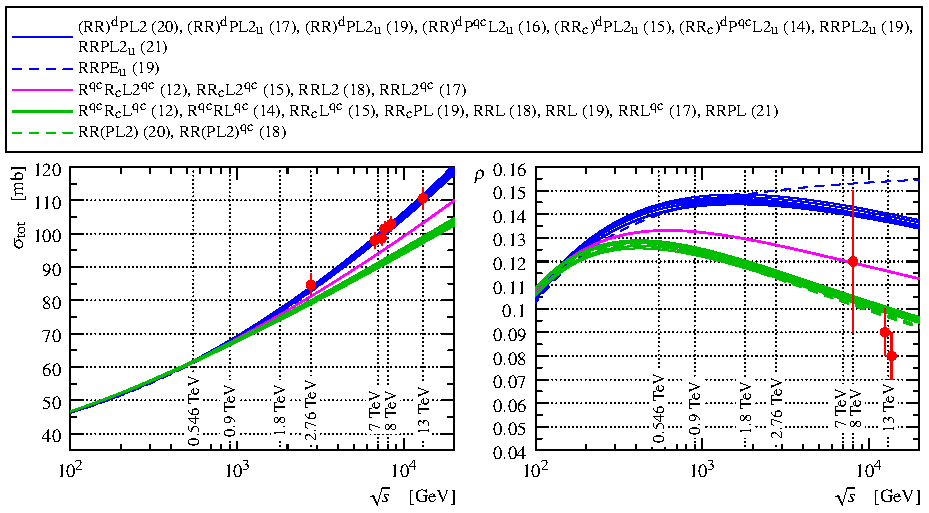
\includegraphics{fig/compete_bands_si_tot_rho.pdf}
\caption{%
\TODO{write}
}
\label{fig:comp bands}
\end{center}
\end{figure*}




\begin{figure*}
\vskip-5mm
\begin{center}
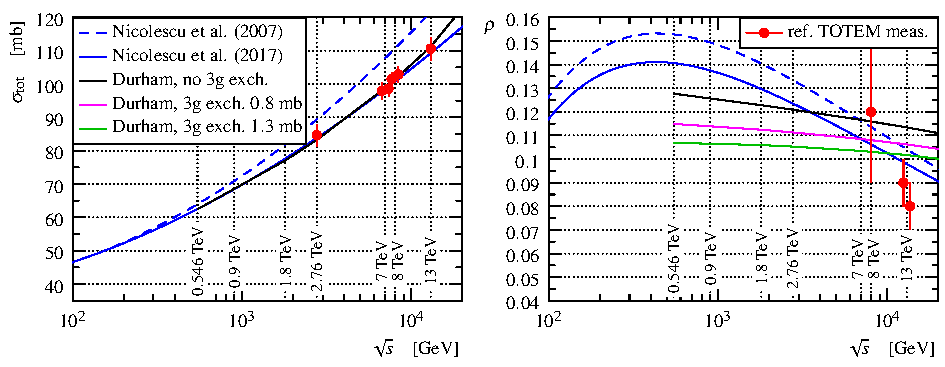
\includegraphics{fig/matching_models_si_tot_rho.pdf}
\caption{%
\TODO{write}
}
\label{fig:match models}
\end{center}
\end{figure*}
